\documentclass[submit]{harvardml}

\course{CS181-S22}
\assignment{Assignment \#6}
\duedate{11:59PM EST, April 29 2022}
\newcommand{\attr}[1]{\textsf{#1}}
\usepackage[OT1]{fontenc}
\usepackage{float}
\usepackage[colorlinks,citecolor=blue,urlcolor=blue]{hyperref}
\usepackage[pdftex]{graphicx}
\usepackage{subfig}
\usepackage{fullpage}
\usepackage{amsmath}
\usepackage{amssymb}
\usepackage{color}
\usepackage{todonotes}
\usepackage{listings}
\usepackage{common}
\usepackage{bm}
\usepackage{enumitem}
\usepackage{tikz}
% \usepackage{xifthen}
\usepackage{soul}
\usepackage{framed}

\usepackage[mmddyyyy,hhmmss]{datetime}

\definecolor{verbgray}{gray}{0.9}

\lstnewenvironment{csv}{
  \lstset{backgroundcolor=\color{verbgray},
  frame=single,
  framerule=0pt,
  basicstyle=\ttfamily,
  columns=fullflexible}}{}

\newcommand{\mueps}{\mu_{\epsilon}}
\newcommand{\sigeps}{\sigma_{\epsilon}}
\newcommand{\mugam}{\mu_{\gamma}}
\newcommand{\siggam}{\sigma_{\gamma}}
\newcommand{\muzp}{\mu_{p}}
\newcommand{\sigzp}{\sigma_{p}}
\newcommand{\gauss}[3]{\frac{1}{2\pi#3}e^{-\frac{(#1-#2)^2}{2#3}}}


\begin{document}
\begin{center}
{\Large Homework 6: Inference in Graphical Models, MDPs}\\
\end{center}

\subsection*{Introduction}

In this assignment, you will practice inference in graphical models as
well as MDPs/RL.  For readings, we recommend \href{http://incompleteideas.net/book/the-book-2nd.html}{Sutton and Barto 2018, Reinforcement Learning: An Introduction}, \href{https://harvard-ml-courses.github.io/cs181-web-2017/}{CS181 2017 Lecture Notes}, and Section 10 and 11 Notes.

Please type your solutions after the corresponding problems using this
\LaTeX\ template, and start each problem on a new page.

Please submit the \textbf{writeup PDF to the Gradescope assignment `HW6'}. Remember to assign pages for each question.

Please submit your \textbf{\LaTeX\ file and code files to the Gradescope assignment `HW6 - Supplemental'}. 

You can use a \textbf{maximum of 2 late days} on this assignment.  Late days will be counted based on the latest of your submissions. 
\\

\newpage

\begin{problem}[Explaining Away + Variable Elimination 15 pts]

  In this problem, you will carefully work out a basic example with
  the ``explaining away'' effect. There are many derivations of this
  problem available in textbooks. We emphasize that while you may
  refer to textbooks and other online resources for understanding how
  to do the computation, you should do the computation below from
  scratch, by hand.

  We have three binary variables: rain $R$, wet grass $G$, and
  sprinkler $S$.
We  assume the following factorization of the joint distribution:
$$
\Pr(R,S,G) = \Pr(R)\Pr(S)\Pr(G\, |\, R, S).
  $$
  
  The conditional probability tables look like the
  following:
  \begin{eqnarray*}
    \Pr(R = 1) &= 0.25 \\
    \Pr(S = 1) &= 0.5 \\
    \Pr(G = 1 | R = 0 , S = 0 ) &= 0 \\
    \Pr(G = 1 | R = 1 , S = 0 ) &= .75 \\
    \Pr(G = 1 | R = 0 , S = 1 ) &= .75 \\
    \Pr(G = 1 | R = 1 , S = 1 ) &= 1
  \end{eqnarray*}
  
 
  \begin{enumerate}
    \item Draw the graphical model corresponding to the
      factorization. Are $R$ and $S$ independent?  [Feel free to use
      facts you have learned about studying independence in graphical models.]
    \item You notice it is raining and check on the sprinkler without
      checking the grass.  What is the probability that it is on?
    \item You notice that the grass is wet and go to check on the
      sprinkler (without checking if it is raining).  What is the
      probability that it is on?
    \item You notice that it is raining and the grass is wet.  You go
      check on the sprinkler.  What is the probability that it is on?
    \item What is the ``explaining away'' effect that is shown above?
    \end{enumerate}
    
Consider if we introduce a new binary variable, cloudy $C$, to the the original three binary variables such that the factorization of the joint distribution is now: 

$$
\Pr(C, R,S,G) = \Pr(C)\Pr(R|C)\Pr(S|C)\Pr(G\, |\, R, S).
$$

\begin{enumerate}
    \setcounter{enumi}{5}
    \item For the marginal distribution $\Pr(R)$, write down the variable elimination expression with the elimination ordering $S, G, C$ (where $S$ is eliminated first, then $G$, then $C$).
    \item For the marginal distribution $\Pr(R)$, write down the variable elimination expression with the elimination ordering $C,G,S$.
    \item Give the complexities for each ordering. Which elimination ordering takes less computation?
\end{enumerate}
\end{problem}

\newpage
\textbf{Solution:}
\begin{enumerate}
    \item 
    Below is the graphical model for this factorization.
    \begin{figure}[H]
        \centering
        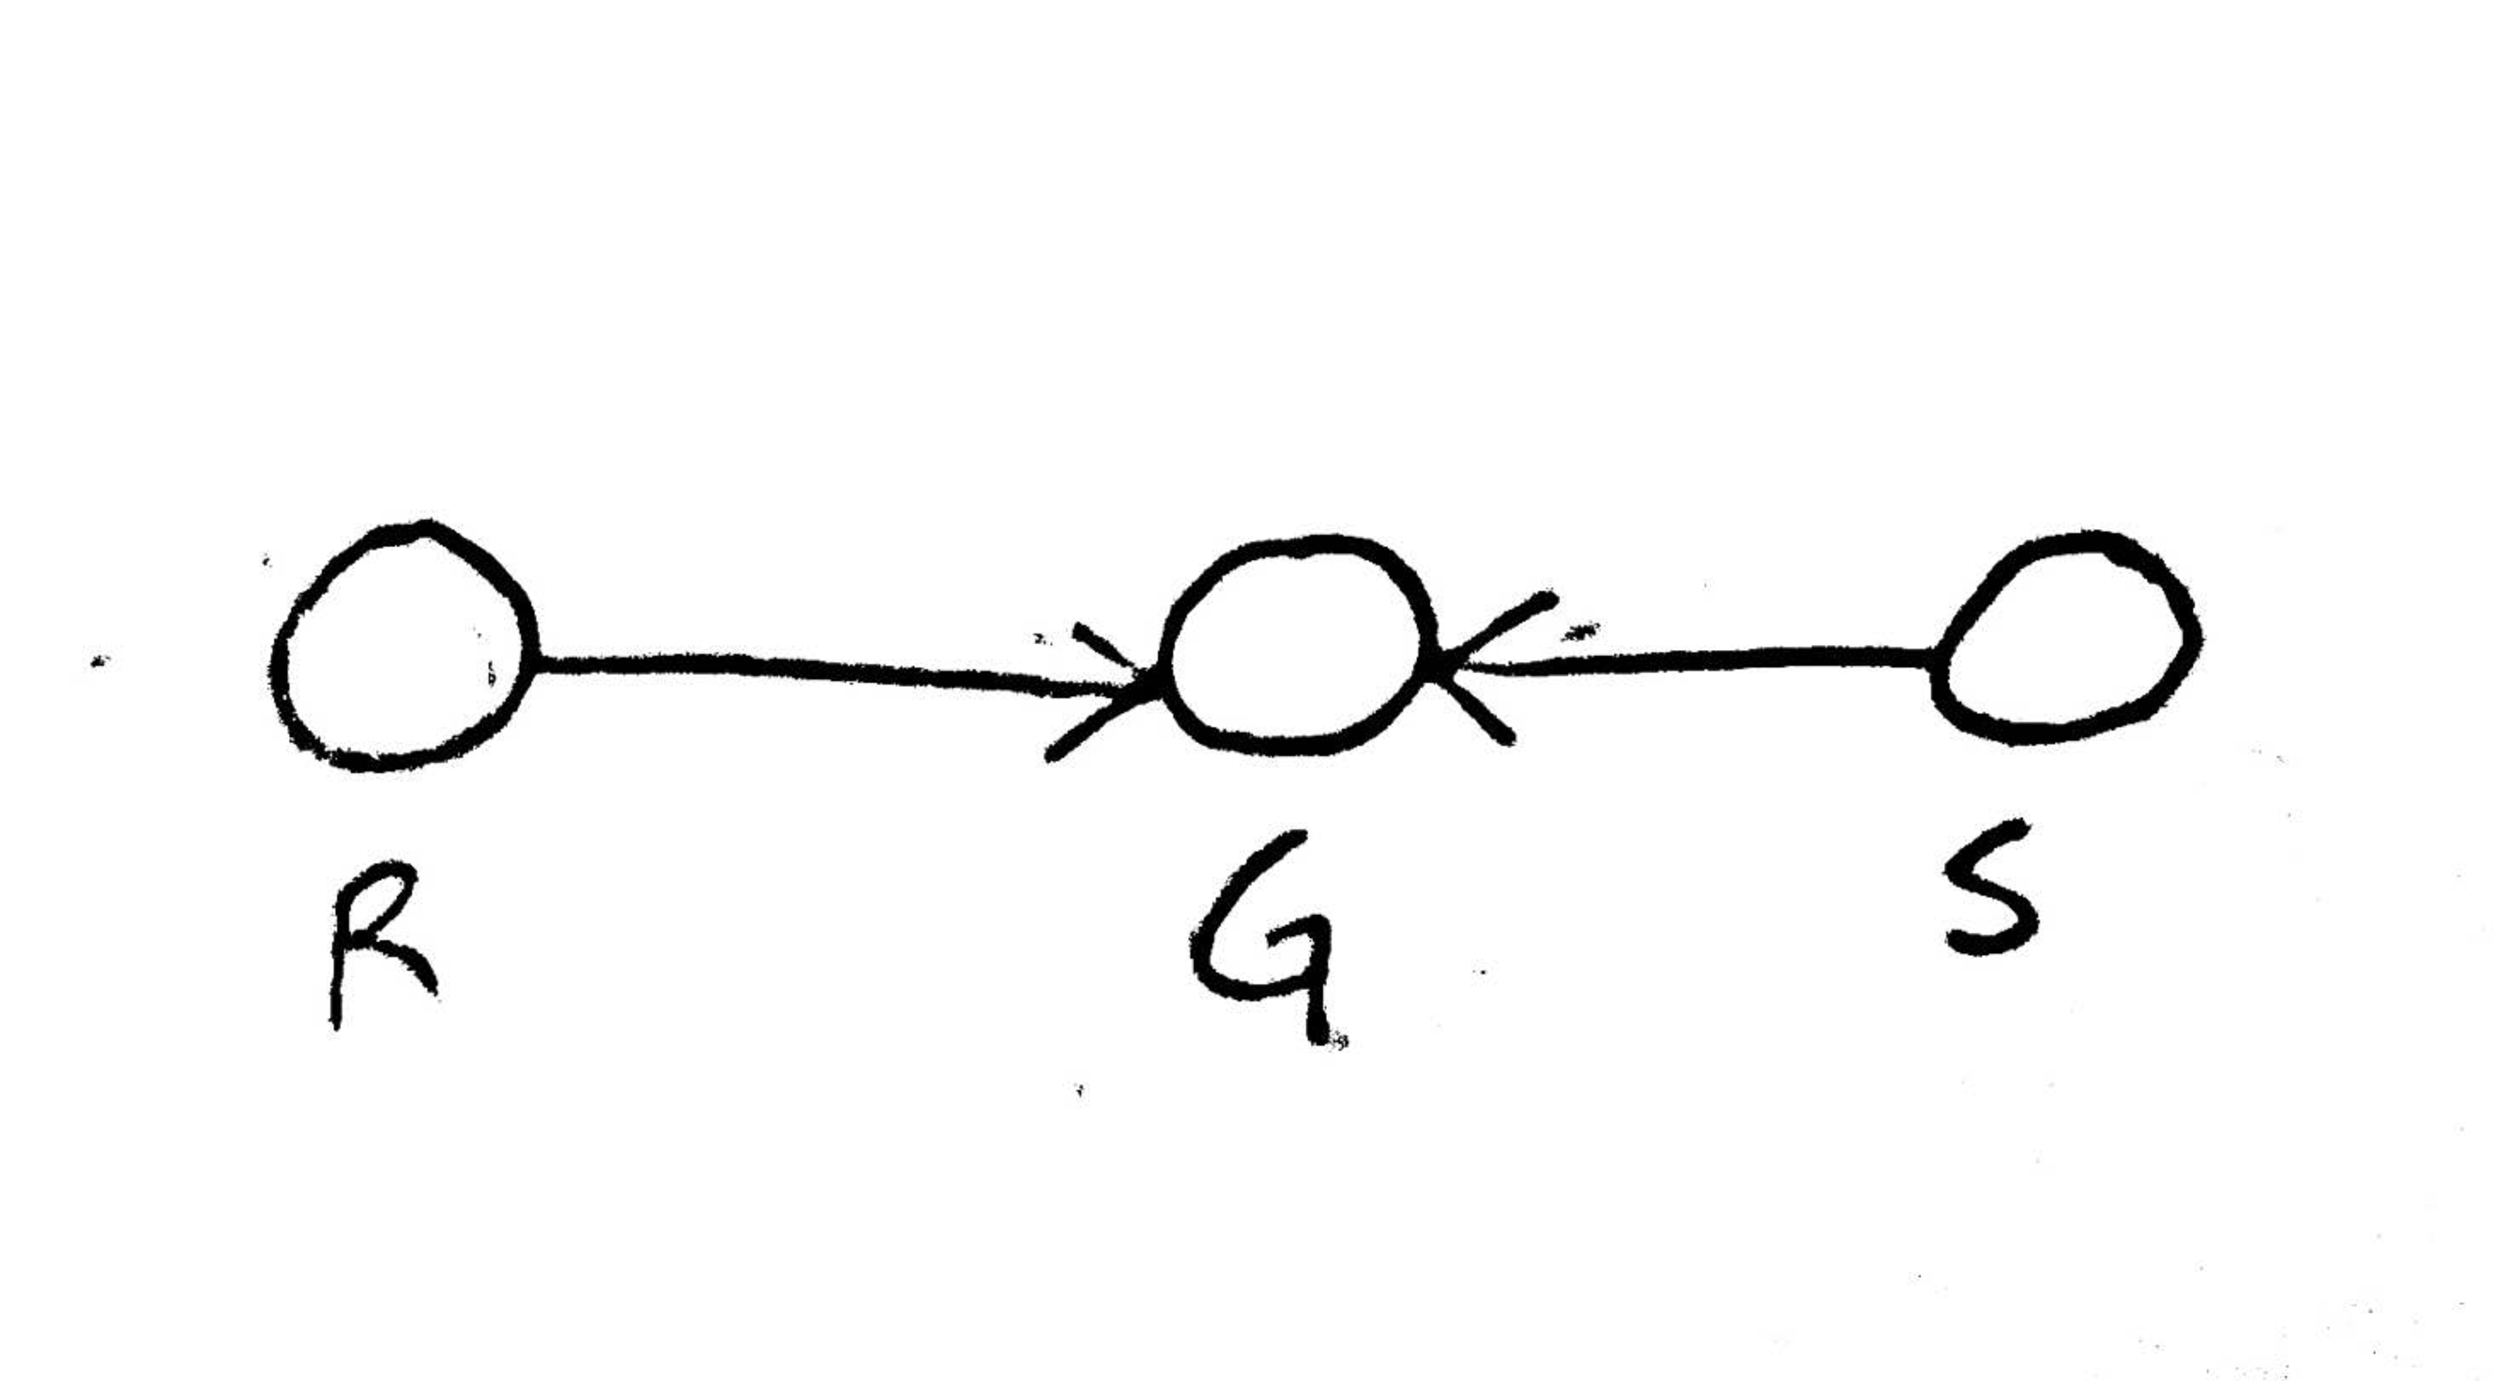
\includegraphics[width=0.5\textwidth]{cs181hw6}
    \end{figure}
    As $G$ is not yet observed,
    $R$ and $S$ are independent.

    \item 
    Given that $R$ and $S$ are independent, the probability that the sprinkler
    is on given that it is raining is 
    $$\boxed{P(S=1|R=1)=P(S=1)=0.5}$$.
    
    \item
    We want to know the probability that the sprinkler is on given that the grass is wet.
    By Bayes' Theorem, we have
    $$P(S=1|G=1)=\frac{P(G=1|S=1)P(S=1)}{P(G=1)}=\frac{P(G=1|S=1)P(S=1)}{P(G=1|S=1)P(S=1)+P(G=1|S=0)P(S=0)}$$

    By the Law of Total Probability, we have
    $$P(G=1|S=1)=P(G=1|R=0,S=1)P(R=0)+P(G=1|R=1,S=1)P(R=1)$$
    $$=(0.75)(1-0.25)+(1)(0.25)=0.8125$$
    $$P(G=1|S=0)=P(G=1|R=0,S=0)P(R=0)+P(G=1|R=1,S=0)P(R=1)$$
    $$=(0)(1-0.25)+(0.75)(0.25)=0.1875$$

    Plugging these back into our definition of $P(S=1|G=1)$ we get
    $$P(S=1|G=1)=\frac{P(G=1|S=1)P(S=1)}{P(G=1|S=1)P(S=1)+P(G=1|S=0)P(S=0)}$$
    $$=\frac{(0.8125)(0.5)}{(0.8125)(0.5)+(0.1875)(0.5)}$$
    $$\boxed{P(S=1|G=1)=0.8125}$$

    \item
    We want to know the probability that the sprinkler is on given that it is raining and the grass
    is wet. By Bayes' Theorem we have
    $$P(S=1|R=1,G=1)=\frac{P(G=1|R=1,S=1)P(S=1|R=1)}{P(G=1|R=1)}$$
    we know that 
    $$P(G=1|R=1,S=1)=1$$
    and that, since R and S are independent, 
    $$P(S=1|R=1)=P(S=1)=0.5$$
    Now, in order to calculate $P(G=1|R=1)$ we use the Law of Total Probability:
    $$P(G=1|R=1)=P(G=1|R=1,S=0)P(S=0)+P(G=1|R=1,S=1)P(S=1)$$
    $$=(0.75)(0.5)+(1)(0.5)=0.875$$
    Plugging these values into our definition of $P(S=1|R=1,G=1)$ we get
    $$P(S=1|R=1,G=1)=\frac{P(G=1|R=1,S=1)P(S=1|R=1)}{P(G=1|R=1)}$$
    $$\boxed{P(S=1|R=1,G=1)=\frac{(1)(0.5)}{(0.875)}\approx 0.571}$$

    \item
    The explaining away effect shown above is that the observance of $G$ makes $R$ a 
    contributor of information to $S$, despite the fact that, before $G$ was observed, $R$ and $S$ were
    completely independent.

    \item
    The marginal distribution $P(R)$ for the $C\rightarrow G\rightarrow S$ ordering is the following
    $$P(R) = \sum_c P(C)P(R|C) \sum_G\sum_S P(G|R,S)P(S|C)$$

    \item
    The marginal distribution $P(R)$ for the $S\rightarrow G\rightarrow C$ ordering is the following
    $$P(R) = \sum_S \sum_G P(G)P(R,S) \sum_C P(C)P(R|C)P(S|C)$$

    \item
    The $C\rightarrow G\rightarrow S$ ordering requires, at its longest step, the calculation of $\sum_S P(G|R,S)P(S|C)$, which requires summing over S for every value 
    in a $k$ by $k$ matrix consisting of all possibilities for $G$ and $C$. This operation has 
    complexity $O(k^3)$. $k$ here refers to the domain size of the variables which in this case is
    2.

    The longest calculation in the $S\rightarrow G\rightarrow C$ ordering, on the other hand, is
    $\sum_C P(C)P(R|C)P(S|C)$. This calculation requires summing over $C$ for every value in a 
    size $k$ vector consisting of all possibilities for $S$. This operation has complexity $O(k^2)$.

    Based on these complexities, the $S\rightarrow G\rightarrow C$ ordering requires less computation.

    Note (confusion on this problem): If we are given $P(R|C)$ and $P(C)$ we can find the distribution 
    $P(R)$ by calculating $\sum_C P(R|C)P(C)$, an operation with complexity $O(k)$. In fact, 
    the methods above involve redundant operations such as $\sum_G P(G|R, C)=1$.

\end{enumerate}
\newpage


\begin{problem}[Policy and Value Iteration, 15 pts]

This question asks you to implement policy and value iteration in a
simple environment called Gridworld.  The ``states'' in Gridworld are
represented by locations in a two-dimensional space.  Here we show each state and its reward:

\begin{center}
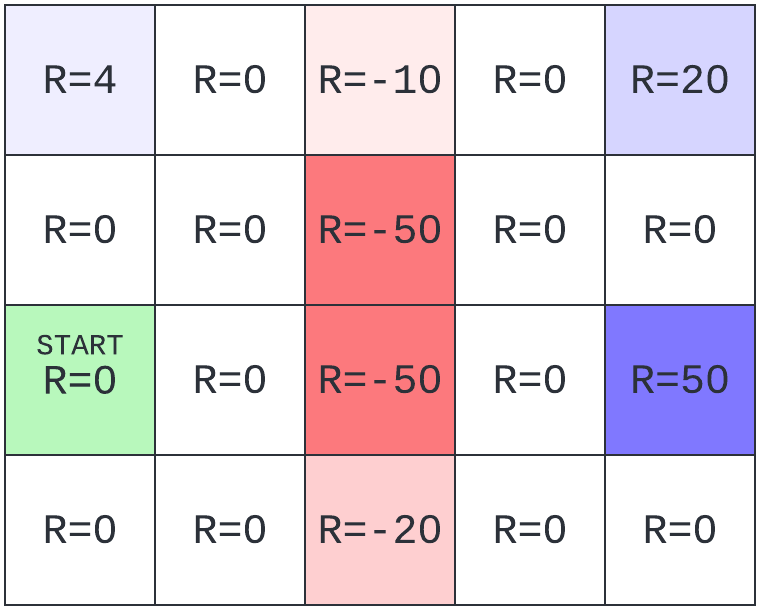
\includegraphics[width=3in]{gridworld.png}
\end{center}
The set of actions is \{N, S, E, W\}, which corresponds to moving north (up), south (down), east (right), and west (left) on the grid.
Taking an action in Gridworld does not always succeed with probability
$1$; instead the agent has probability $0.1$ of ``slipping'' into a
state on either side, but not backwards.  For example, if the agent tries to move right from START, it succeeds with probability 0.8, but the agent may end up moving up or down with probability 0.1 each. Also, the agent cannot move off the edge of the grid, so moving left from START will keep the agent in the same state with probability 0.8, but also may slip up or down with probability 0.1 each. Lastly, the agent has no chance of slipping off the grid - so moving up from START results in a 0.9 chance of success with a 0.1 chance of moving right.

Also, the agent does not receive the reward of a state immediately upon entry, but instead only after it takes an action at that state. For example, if the agent moves right four times (deterministically, with no chance of slipping) the rewards would be +0, +0, -50, +0, and the agent would reside in the +50 state. Regardless of what action the agent takes here, the next reward would be +50.

Your job is to implement the following three methods in file \texttt{T6\_P2.ipynb}. Please use the provided helper functions \texttt{get\_reward} and \texttt{get\_transition\_prob} to implement your solution.

\emph{Do not use any outside code.  (You may still collaborate with others according to the standard collaboration policy in the syllabus.)}  

\emph{Embed all plots in your writeup.}
\end{problem}
\newpage

\begin{framed}
\textbf{Problem 2} (cont.)\\

\textbf{Important: } The state space is represented using integers, which range from 0 (the top left) to 19 (the bottom right). Therefore both the policy \texttt{pi} and the value function \texttt{V} are 1-dimensional arrays of length \texttt{num\_states = 20}. Your policy and value iteration methods should only implement one update step of the iteration - they will be repeatedly called by the provided \texttt{learn\_strategy} method to learn and display the optimal policy. You can change the number of iterations that your code is run and displayed by changing the $\texttt{max\_iter}$ and $\texttt{print\_every}$ parameters of the $\texttt{learn\_strategy}$ function calls at the end of the code.

Note that we are doing infinite-horizon planning to maximize the expected reward of the traveling agent. For parts 1-3, set discount factor $\gamma = 0.7$.

\begin{itemize}
    \item[1a.]  Implement function \texttt{policy\_evaluation}.  Your
      solution should learn value function $V$, either using a closed-form expression or iteratively using
      convergence tolerance $\texttt{theta = 0.0001}$ (i.e., if
      $V^{(t)}$ represents $V$ on the $t$-th iteration of your policy
      evaluation procedure, then if $|V^{(t + 1)}[s] - V^{(t)}[s]|
      \leq \theta$ for all $s$, then terminate and return $V^{(t + 1)}$.)

    \item[1b.] Implement function \texttt{update\_policy\_iteration} to update the policy \texttt{pi} given a value function \texttt{V} using \textbf{one step} of policy iteration.
    
    \item[1c.] Set \texttt{max\_iter = 4}, \texttt{print\_every = 1} to show the learned value function and the associated policy for the first 4 policy iterations. Do not modify the plotting code. Please fit all 4 plots onto one page of your writeup.
    
    \item [1d.] Set \texttt{ct = 0.01} and increase \texttt{max\_iter} such that the algorithm converges. Include a plot of the final learned value function and policy. How many iterations does it take to converge? Now try \texttt{ct = 0.001} and \texttt{ct = 0.0001}. How does this affect the number of iterations until convergence?
      
    \item [2a.] Implement function
      \texttt{update\_value\_iteration}, which performs \textbf{one step} of value iteration to update \texttt{V}, \texttt{pi}.
      
    \item [2b.] Set \texttt{max\_iter = 4}, \texttt{print\_every = 1} to show the learned value function and the associated policy for the first 4 value iterations. Do not modify the plotting code. Please fit all 4 plots onto one page of your writeup.
    
    \item [2c.] Set \texttt{ct = 0.01} and increase \texttt{max\_iter} such that the algorithm converges. Include a plot of the final learned value function and policy. How many iterations does it take to converge? Now try \texttt{ct = 0.001} and \texttt{ct = 0.0001}. How does this affect the number of iterations until convergence?
    
    \item[3] Compare and contrast the number of iterations, time per iteration, and overall runtime between policy iteration and value iteration. What do you notice?
    
    \item[4] Plot the learned policy with each of $\gamma \in (0.6,0.7,0.8,0.9)$. Include all 4 plots in your writeup. Describe what you see and provide explanations for the differences in the observed policies. Also discuss the effect of gamma on the runtime for both policy and value iteration.
    
    \item[5] Now suppose that the game ends at any state with a positive reward, i.e. it immediately transitions you to a new state with zero reward that you cannot transition away from. What do you expect the optimal policy to look like, as a function of gamma? Numerical answers are not required, intuition is sufficient.
 
\end{itemize}
\end{framed}

\newpage
\textbf{Solution:}
\begin{itemize}
    \item[1a.]
    Implemented in \texttt{T1.P2.ipynb}.

    \item[1b.]
    Implemented in \texttt{T1.P2.ipynb}.

    \item[1c.]
    Below are the plots resulting from setting \texttt{max\_iter = 4}, \texttt{print\_every = 1}.

    \begin{figure}[H]
        \centering
        {
            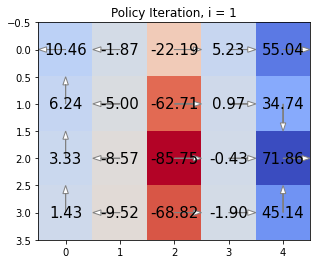
\includegraphics[width=0.48\textwidth]{hw6_1c_1}
            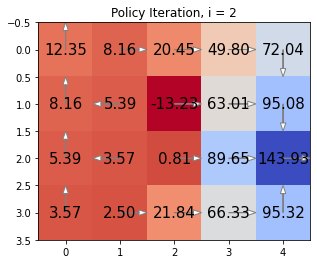
\includegraphics[width=0.48\textwidth]{hw6_1c_2}
        }\hfill
        {
            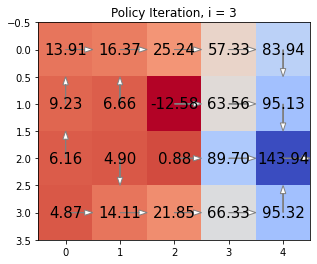
\includegraphics[width=0.48\textwidth]{hw6_1c_3}
            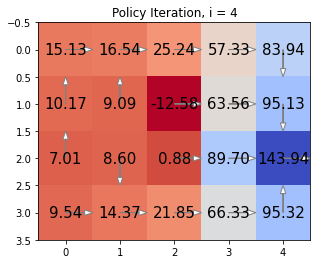
\includegraphics[width=0.48\textwidth]{hw6_1c_4}
        }
    \end{figure}

    \item[1d.]
    With \texttt{ct = 0.01} and \texttt{max\_iter = 100}, the final learned value function is the 
    following:

    \begin{figure}[H]
        \centering
        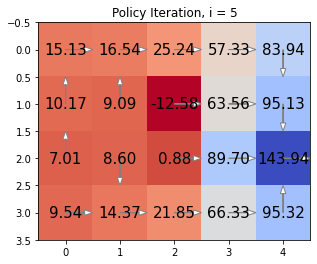
\includegraphics[width=0.48\textwidth]{hw6_1d}
    \end{figure}

    This final learned value function takes 5 iterations to converge. Using 
    \texttt{ct = 0.001} does not affect the number of iterations until convergence.
    Neither does using \texttt{ct = 0.0001}.
    
    \item[2a.]
    Implemented in \texttt{T1.P2.ipynb}.
    
    \item[2b.]
    Below are the plots resulting from setting \texttt{max\_iter = 4}, \texttt{print\_every = 1}.

    \begin{figure}[H]
        \centering
        {
            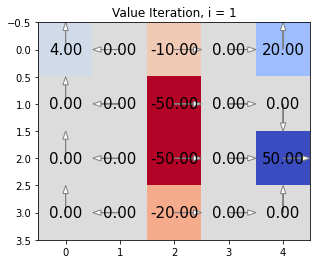
\includegraphics[width=0.48\textwidth]{hw6_2b_1}
            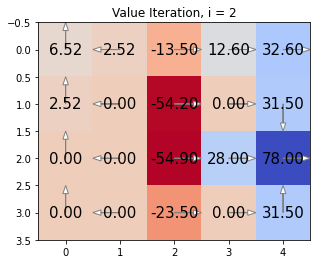
\includegraphics[width=0.48\textwidth]{hw6_2b_2}
        }\hfill
        {
            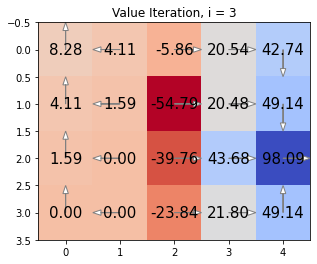
\includegraphics[width=0.48\textwidth]{hw6_2b_3}
            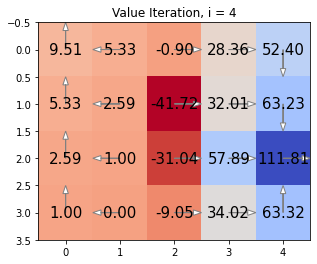
\includegraphics[width=0.48\textwidth]{hw6_2b_4}
        }
    \end{figure}
    
    \item[2c.]
    With \texttt{ct = 0.01} and \texttt{max\_iter = 100}, the final learned value function is the 
    following:
    \begin{figure}[H]
        \centering
        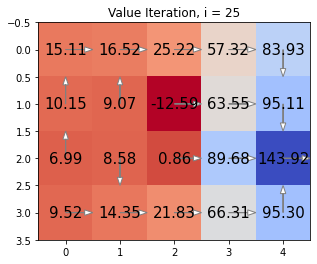
\includegraphics[width=0.48\textwidth]{hw6_2c}
    \end{figure}
    This final learned value function takes 25 iterations to converge. Using 
    \texttt{ct = 0.001} changes this to 31 iterations.
    Using \texttt{ct = 0.0001} changes this to 38 iterations.
    
    \item[3.]
    Policy iteration requires less iterations and takes considerably more time 
    per iteration.
    Value iteration requires more iterations and takes considerably less time 
    per iteration. 
    Overall, the tradeoff between number of iterations for each and time per iteration 
    cancels out and both methods have a very similar overall runtime.

    One important thing to note, however, is that Value Iteration is sensitive 
    to the setting for convergence tolerance while Policy Iteration is not.
    If we want to reach a small convergence tolerance (e.g. \texttt{ct = 0.0001}), then Value Iteration
    takes more iterations and results in a much higher overall runtime as compared
    with Policy Iteration.

    \item[4.]
    We include the plot below. Policy Iteration was used to calculate these.
    \begin{figure}[H]
        \centering
        {
            \subfloat[$\gamma=0.6$]{
                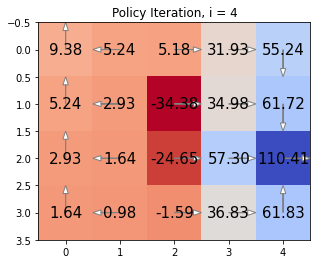
\includegraphics[width=0.48\textwidth]{hw6_4_6}
            }
            \subfloat[$\gamma=0.7$]{
                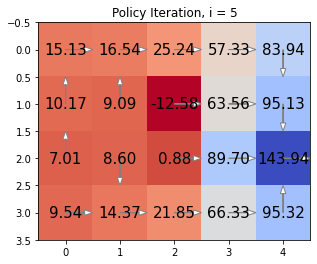
\includegraphics[width=0.48\textwidth]{hw6_4_7}
            }
        }\hfill
        {
            \subfloat[$\gamma=0.8$]{
                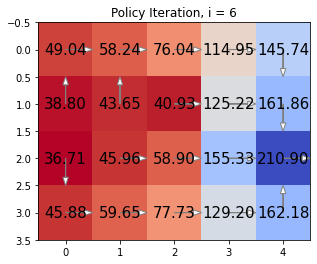
\includegraphics[width=0.48\textwidth]{hw6_4_8}
            }
            \subfloat[$\gamma=0.9$]{
                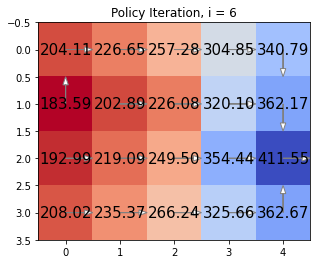
\includegraphics[width=0.48\textwidth]{hw6_4_9}
            }
        }\caption{Learned policies with differing discount values ($\gamma$)}
    \end{figure}
    
    \item[5.]       
    I would expect the optimal policy to, depending on how high gamma is, favor
    avoiding the squares with reward 4 and 20 in order to prioritize reaching the
    square with reward 50. With lower values of gamma, the policy will feel fine
    reaching the squares with the lower positive rewards, and the policy may not look 
    too different from its corresponding policy in the regular game. With high
    values for gamma, however, it will definitely avoid these lower positive reward value squares.
\end{itemize}



\begin{problem}[Reinforcement Learning, 20 pts]
  In 2013, the mobile game \emph{Flappy Bird} took the world by storm. You'll be developing a Q-learning agent to play a similar game, \emph{Swingy Monkey} (See Figure~\ref{fig:swingy}).  In this game, you control a monkey that is trying to swing on vines and avoid tree trunks.  You can either make him jump to a new vine, or have him swing down on the vine he's currently holding.  You get points for successfully passing tree trunks without hitting them, falling off the bottom of the screen, or jumping off the top.  There are some sources of randomness: the monkey's jumps are sometimes higher than others, the gaps in the trees vary vertically, the gravity varies from game to game, and the distances between the trees are different.  You can play the game directly by pushing a key on the keyboard to make the monkey jump.  However, your objective is to build an agent that \emph{learns} to play on its own. 
  
   You will need to install the \verb|pygame| module
  (\url{http://www.pygame.org/wiki/GettingStarted}).
  

\textbf{Task:}
Your task is to use Q-learning to find a policy for the monkey that can navigate the trees.  The implementation of the game itself is in file \verb|SwingyMonkey.py|, along with a few files in the \verb|res/| directory.  A file called \verb|stub.py| is the starter code for setting up your learner that interacts with the game.  This is the only file you need to modify (but to speed up testing, you can comment out the animation rendering code in \verb|SwingyMonkey.py|). You can watch a YouTube video of the staff Q-Learner playing the game at \url{http://youtu.be/l4QjPr1uCac}.  It figures out a reasonable policy in a few dozen iterations.
You'll be responsible for implementing the Python function  \verb|action_callback|. The action callback will take in a dictionary that describes the current state of the game and return an action for the next time step.  This will be a binary action, where 0 means to swing downward and 1 means to jump up.  The dictionary you get for the state looks like this:
\begin{csv}
{ 'score': <current score>,
  'tree': { 'dist': <pixels to next tree trunk>,
            'top':  <height of top of tree trunk gap>,
            'bot':  <height of bottom of tree trunk gap> },
  'monkey': { 'vel': <current monkey y-axis speed>,
              'top': <height of top of monkey>,
              'bot': <height of bottom of monkey> }}
\end{csv}
All of the units here (except score) will be in screen pixels. Figure~\ref{fig:swingy-ann} shows these graphically. 
Note that since the state space is very large (effectively continuous), the monkey's relative position needs to be discretized into bins. The pre-defined function \verb|discretize_state| does this for you.

\textbf{Requirements}
\\
\textit{Code}: First, you should implement Q-learning with an
$\epsilon$-greedy policy yourself. You can increase the performance by
trying out different parameters for the learning rate $\alpha$,
discount rate $\gamma$, and exploration rate $\epsilon$. \emph{Do not use outside RL code for this assignment.} Second, you should use a method of your choice to further improve the performance. This could be inferring gravity at each epoch (the gravity varies from game to game), updating the reward function, trying decaying epsilon greedy functions, changing the features in the state space, and more. One of our staff solutions got scores over 800 before the 100th epoch, but you are only expected to reach scores over 50 before the 100th epoch. {\bf Make sure to turn in your code!} \\\\
\textit{Evaluation}: In 1-2 paragraphs, explain how your agent performed and what decisions you made and why. Make sure to provide evidence where necessary to explain your decisions. You must include in your write up at least one plot or table that details the performances of parameters tried (i.e. plots of score vs. epoch number for different parameters).
\\\\
\textit{Note}: Note that you can simply discretize the state and action spaces and run the Q-learning algorithm. There is no need to use complex models such as neural networks to solve this problem, but you may do so as a fun exercise.

\end{problem}
\begin{figure}[H]
    \centering%
    \subfloat[SwingyMonkey Screenshot]{%
        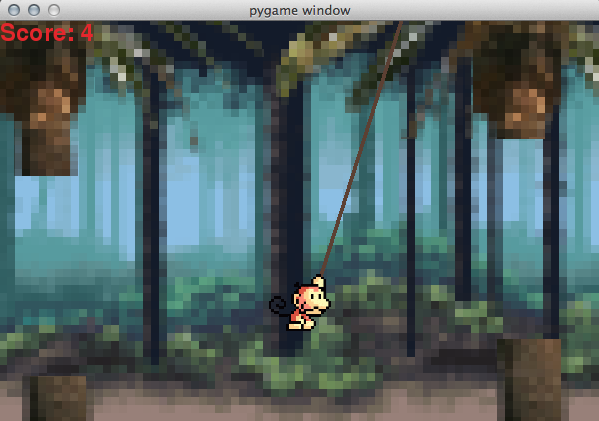
\includegraphics[width=0.48\textwidth]{figures/swingy}
        \label{fig:swingy}
    }\hfill
    \subfloat[SwingyMonkey State]{%
        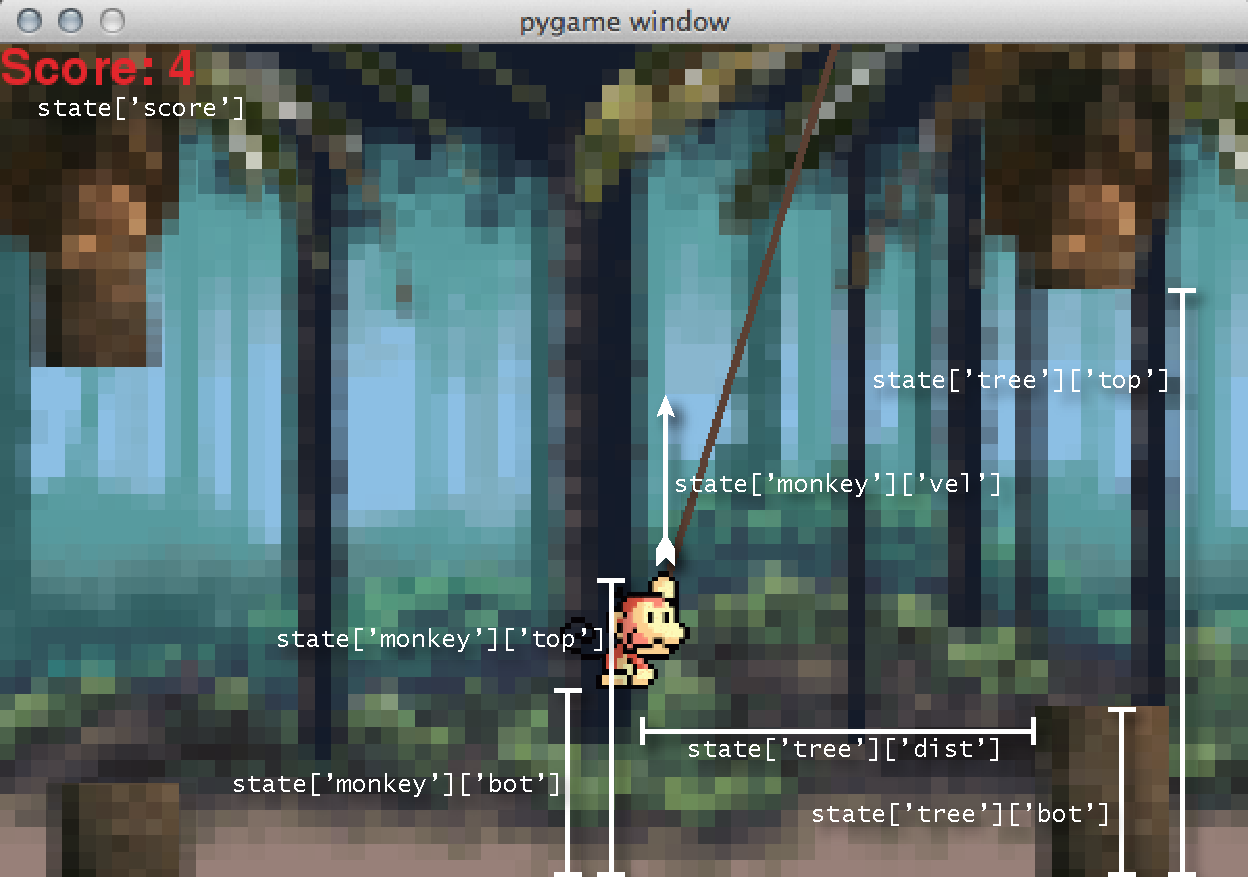
\includegraphics[width=0.48\textwidth]{figures/swingy-ann}
        \label{fig:swingy-ann}
    }
    \caption{(a) Screenshot of the Swingy Monkey game.  (b) Interpretations of various pieces of the state dictionary.}
\end{figure}
    
\textbf{Solution:}

\newpage
\newpage
%%%%%%%%%%%%%%%%%%%%%%%%%%%%%%%%%%%%%%%%%%%%%
% Name and Calibration
%%%%%%%%%%%%%%%%%%%%%%%%%%%%%%%%%%%%%%%%%%%%%
\newpage
\subsection*{Name}
Rodney Lafuente Mercado
\subsection*{Collaborators and Resources}
Whom did you work with, and did you use any resources beyond cs181-textbook and your notes?
\subsection*{Calibration}
Approximately how long did this homework take you to complete (in hours)? 
\end{document}